\documentclass[10pt]{article}
\usepackage[frenchb]{babel}
\usepackage[utf8x]{inputenc}
\usepackage[T1]{fontenc}
\usepackage{lmodern}
\usepackage{amsthm}

\usepackage{color}
\usepackage{multirow}
%\usepackage{fourier-orns}
\usepackage{hyperref}
\usepackage[margin=3.2cm, top=2cm, bottom=2cm,left=2cm,a4paper]{geometry}
\usepackage{graphicx}
\usepackage{caption}
\usepackage{array}


\setlength{\parskip}{2mm}
\setlength{\parindent}{0pt}

\usepackage{enumitem}
\setlist[itemize]{noitemsep, topsep=0pt}

\newcounter{questionum}
\setcounter{questionum}{0}

\newcommand\com[1]{\textsf{#1}}

\newcommand\question[1]{\par\noindent\textbf{\thequestionum}.~#1\addtocounter{questionum}{1}}
\let\oldmarginpar\marginpar
\renewcommand\marginpar[1]{\oldmarginpar{\tiny#1}}

\makeatletter
\renewcommand\maketitle{\begin{minipage}[c]{.7\textwidth}%
{\LARGE\sf \@title}
\\[1ex] \today
\end{minipage}
\hfill
\begin{minipage}[c]{.2\textwidth}

\includegraphics[width=\textwidth]{grid-0}
\end{minipage}
}
\makeatother


\title{Maîtriser l'application web Vidjil:\\ Analyser et interagir avec les  clones
}

\begin{document}
\maketitle

  \textit{Le but de cette session pratique est d'apprendre comment
  visualiser, filtrer, analyser et regrouper les clones de l'application web
  Vidjil. %
Ces clones ont pu être calculés avec l'algorithme de la plateforme Vidjil ou par n'importe
quel autre algorithme.}

\bigskip

\question{Connectez-vous au serveur public (\url{https://app.vidjil.org}), soit avec votre compte
ou avec le compte de démonstration (\texttt{demo@vidjil.org} / \texttt{demo}),
sélectionnez le patient \textit{Demo LIL-L3 (tutorial)} patient, et cliquez sur le lien en bas à droite
``see results: multi''.
L'application web Vidjil s'ouvre.
}

Ce patient (patient 063 de \href{http://dx.doi.org/10.1016/j.leukres.2016.11.009}{Étude de Lille sur la faisabilité de la MRD en utilisant le séquençage à haut débit})
souffre d'une T-ALL. Nous avons un échantillon de diagnostic,
avec des clones dominants en IGH et TRG,
et quatre échantillons de suivi, incluant une rechute.

\question{Dans le menu \com{settings}, essayez les différentes options de \com{sample key}.
Les cinq échantillons peuvent être annotés par leur nom, leur date d'échantillonnage
ou par le nombre de jours depuis la date du premier échantillon.
}

Dans la section suivante, nous nous focalisons sur l'échantillon de diagnostic.
La section~\ref{sec:tracking} concernera la comparaison de plusieurs échantillons.



\section{Évaluation de la qualité d'un run et de l'analyse}
L'application web Vidjil permet d'exécuter plusieurs algorithmes ``RepSeq'' (analyse de répertoires immunologiques).
Chaque algorithme ReqSeq a sa propre définition de ce qu'est un clone
(ou, plus précisement, un clonotype),
et de comment analyser chaque read et leur assigner une désignation V(D)J.
Le nombre de reads analysées dépent de l'algorithme utilisé.
Cet échantillon a été traité par l'algorithme de Vidjil.


\marginpar{Le pourcentage de reads analysées peut varier de 0,01\,\% (voire
  moins, pour du
  RNA-Seq ou de la capture) à 98--99\,\% (pour des séquençages de très bonne
  qualité, généralement sur séquenceurs Illumina)}

\question{Combien de reads ont été analysées dans l'échantillon en cours~?}

Nous allons essayer de comprendre pourquoi certains reads n'ont pas été
analysées dans notre échantillon. Cela pourrait refléter un problème
pendant le protocole de séquençage\ldots{} ou être normal.
Nous cliquons sur le «~i~» dans la partie en haut à gauche pour accéder à la boîte
d'information sur l'échantillon en cours.

\question{Quelle est la longueur moyenne des reads sur les IGH~? et sur les
  TRG~? Les lignes commençant par UNSEG donnent les raisons pour lesquelles
  certains reads n'ont pas été analysées.
  Vous pouvez voir ce que signifient ces raisons dans la documentation en ligne de l'algorithme : 
  \href{http://www.vidjil.org/doc/vidjil-algo\#unsegmentation-causes}{vidjil.org/doc/vidjil-algo\#unsegmentation-causes
  }
\question{Quelles sont les principales causes expliquant que les reads n'ont pas
  été analysées~? Regardez aussi la longueur moyenne des reads non
  analysées. Observez-vous quelque chose de particulier au niveau de la
  longueur moyenne de ces reads~?}

\section{Visualiser et filtrer les clones}

\subsection{Visualiser les clones}

Dan ce fichier, le clone le plus abondant est \texttt{IGHV3-9 7/CCCGGA/17 J6*02}.

\question{Sélectionnez ce clone, en cliquant sur la liste ou la grille/
Combien de reads ce clone représente-t-il ?
(voir en bas à droite)
}

Il y a plusieurs manières d'afficher la désignation V(D)J.

\question{Dans le menu \textit{settings}, sélectionner \com{length}
pour afficher les zones N en fonction de leur taille.
Revenez à la situation initiale grâce au réglage \com{sequence (when short)} pour afficher en entier les séquences N (quand elles sont courtes).}

\question{Essayez aussi les options \com{alleles in clone names} : 
en sélectionnant \com{always}, le gène V est affiché comme \com{IGHV3-9*01}.
Revenez à la situation intitale avec \com{when not *01} pour avoir des désignations V(D)J plus compactes.}


\subsection{Montrer plus de clones}

Par défaut, Vidjil affiche les 50 clones les plus abondants \textit{(top 50)}
pour chaque échantillon ou point de MRD. Avec 5 points de suivi, nous
pouvons donc avoir entre 50 et 250 clones observables, tout dépend si le
\textit{top 50} reste le même pour tous les points ou s'il varie.
Ce nombre
minimum peut être augmenté jusqu'à 100 en allant dans le menu \com{filter} et en
poussant vers la droite le curseur.

\question{Observez comment change la taille cumulée des petits clones IGH («~smaller
  clones~»). Quelle était la valeur initiale~? Quelle est-elle
  maintenant~?}
 Les «~smaller clones~» correspondent aux clones qui n'ont
  pas été séparément analysés car ils ne sont jamais parmi les plus abondants.


\subsection{Taguer et filtrer les clones}

Considérons les clones les plus abondants de la liste :
\texttt{IGHV3-9 7/CCCGGA/17 J6*02} et \texttt{TRGV10 13//5 JP1}.
Il serait intéressant de pouvoir les étiqueter pour s'en souvenir plus tard.

\question{Cliquez sur l'étoile à côté de ces clones et choisissez des catégories
telles que \texttt{clone 1} ou \texttt{clone 2}. Observez comment la couleur s'applique dans toutes les parties de l'application.}

Lorsque des clones ont été étiquetés, il est ensuite possible de
les filtrer selon les couleurs choisies.

\question{Dans la partie en haut à gauche, cliquez sur le carré gris (à droite
  de la liste des carrés de couleur). Que se passe-t-il~? Et si vous
  recliquez encore~?}

C'est un moyen de filtrer certains clones. Cela peut être utile si vous
voulez vous focaliser sur quelques clones spécifiques. Il est également
possible de filtrer ces clones, soit par leur nom, soit par leur séquence
d'ADN.

\question{Dans le champ de recherche, entrez la séquence \texttt{GGAGTCGGGG} et validez
  la recherche par la touche Entrée. Combien de séquences ont été
  retirées~?} 
À noter, la recherche se fait à la fois sur les brins sens
  et antisens.
\question{Vérifiez si cela est vrai en recherchant maintenant la séquence
  réverse complémentaire~: \texttt{CCCCGACTCC}. Trouvez-vous le même résultat que
  précédemment~?}
\question{Comment pouvez-vous annuler ce filtre et revoir l'ensemble des
  clones~?}

\bigskip

Une autre façon de signaler un clone spécifique est de le renommer.

\question{Double-cliquez sur le nom d'un clone (parmi la liste des clones) et
  lui choisir un autre nom (comme par exemple «~clone principal~»). Validez cette action
  par la touche Entrée.}

\bigskip

Après ce renommage, vous pouvez voir que ce clone est déjà sélectionné.

\question{Cliquez sur plusieurs clones en maintenant la touche \texttt{Ctrl} enfoncée
  pour conserver la sélection. A chaque ajout d'un clone, sa séquence
  apparaît dans l'encart du bas.}
\question{
  Combien de clones ont été sélectionnés~? Combien de reads cela
  représente-t-il~? (Regarder à droite dans l'encart du bas.)}
\question{Quand vous voulez vous focaliser sur des clones sélectionnés, vous
  pouvez cliquer sur le lien \com{(focus)} sur la droite de l'encart du bas
  (à droite du nombre de clones sélectionnés).
  Cela est pratique lorsque vous souhaitez analyser quelques clones parmi de
  nombreux autres sans être gêné par ces autres clones.}
\question{%
  Pour retirer ce focus, cliquez sur la croix située à droite du champ
  de recherche.}
\question{%
  Pour tout désélectionner, vous pouvez cliquer sur une zone vide de
  la grille des clones.} % encart haut ou bas.}

Parfois, on souhaite cacher des clones provenant d'un bruit de fond.

\question{Sélectionnez un clone ou plusieurs clones et cliquez sur \com{hide}, à côté de  \com{focus}.
  Rendez ces clones à nouveau visible en cliquant sur la croix à droite du champ de recherche.}
 

\section{Analyse de populations clonales}

\subsection{Regroupement de clones («~cluster~») par l'inspection de leur
    séquence}

La première chose à faire est de voir si certains clones peuvent et
doivent être <<~regroupés~>> (du fait d'erreurs de PCR ou de séquençage).
Cette étape peut être automatisée mais cela n'enlève pas la
nécessité d'une vérification de ce regroupement par un œil expert.

Par défaut, dans l'encart de visualisation graphique des clones
(«~grille~»), les clones apparaissent classés selon leurs gènes V et J
ou plus généralement selon les gènes 5' et 3'.

\question{Identifiez dans la grille les clones avec la recombinaison
  \textit{IGHV-3-11}-\textit{IGHJ6} et sélectionnez-les. Vous pouvez utiliser la touche \texttt{Ctrl}, mais aussi les
  sélectionner en dessinant un rectangle autour des clones souhaités en
  maintenant le bouton gauche de la souris appuyé.}

Les séquences des clones apparaissent désormais dans l'encart du bas
(«~segmenteur~»). Si beaucoup de clones ont été sélectionnés, il est
possible de voir toutes les séquences en faisant glisser la souris dans
le segmenteur (l'encart s'agrandit). Les séquences dans ce segmenteur
peuvent être comparées visuellement mais il est aussi possible de les
aligner pour voir plus facilement les similarités.
\question{Cliquez sur le bouton \com{align} dans la partie en bas à gauche. Les
  différences sont mises en exergue par un changement de style (gras et
  couleur brique).}

Il en va de l'expertise de l'utilisateur et du cas d'utilisation pour déterminer si le degré de
similarité entre les clones du segmenteur est suffisant pour un éventuel
regroupement. Si certaines séquences ne semblent pas suffisamment homologues,
vous pouvez les retirer du segmenteur en cliquant sur la croix devant la
séquence (partie à gauche du segmenteur).

\question{Retirez toutes les séquences qui ne sont pas assez proches de la
  première.}

Maintenant toutes les séquences du segmenteur doivent être hautement
similaires. Les différences observées ne doivent être dues qu'à des
erreurs de séquençage ou de PCR. Ces artefacts (mutations,
homopolymères, insertions, délétions) sont dépendants du séquenceur
utilisé et de la technique de PCR.

\question{Regroupez tous les clones en un seul en cliquant sur le bouton \com{cluster}
  puis sur le bouton \com{align}.}

Toutes les séquences ainsi regroupées apparaissent sous un seul et même
clone. Dans la liste des clones, c'est repérable~: le clone qui contient
les sous-clones apparaît avec un $+$ sur la gauche. Vous pouvez
cliquer sur ce $+$ pour avoir la liste des sous-clones qui compose le
clone issu du regroupement.

\question{Cliquez sur le $+$ et observez les changements dans la grille.}

Comme vous avez pu le constater, les sous-clones apparaissent encore sur
le graphe. Vous pouvez encore les comparer si vous le voulez (par
exemple pour vérifier si le regroupement est correct ou non) et si nécessaire
vous pouvez toujours retirer certains sous-clones du regroupement par la croix
à gauche de la liste.

\question{Juste pour l'exercice, retirez le dernier clone de la liste du
segmenteur.}

\question{Ouvrez le menu \com{cluster}, et choisissez l'optin \com{cluster by V/5}.
Que s'est-il passé ? 
Il y a maintenant dex clones avec TRGV2. Pourquoi ?}

\question{Dans le menu \com{cluster}, sélectionnez \com{revert to previous cluster} pour annuler le groupe.}



\subsection{Autres paramètres et analyses des clones}

Pour déterminer les homologies de séquences, nous avons utilisé
les gènes V et J. Toutefois, il existe d'autres façons de
rechercher les similitudes entre les séquences, parfois plus
pertinentes. De même, vous pourriez vouloir afficher d'autres paramètres
de visualisation de la population lymphocytaire. Pour l'exemple, nous
allons afficher les clones selon les gènes V versus la longueur
des N insérés.

\question{Dans le menu \com{plot} (coin haut gauche de la grille),
  dans le champ \com{preset}, sélectionnez \com{V/N length}. Vous pouvez
  continuer de regrouper les clones en les alignant puis en cliquant sur
  \com{cluster} si besoin.}
\question{%
  Vous pouvez aussi utiliser le preset \com{clone consensus
  length/GC content} qui a tendance à  bien séparer les clones distincts.}

Notez que vous pouvez modifier directement les axes du graphe, en ouvrant le
menu \com{plot} et en sélectionnant les axes $x$ et $y$.
Dans la visualisation en histogramme, la taille des
rectangle dépend toujours de la taille des clones, et l'axe $y$ règle l'ordre
des rectangles pour chaque même $x$.

\question{Dans le menu \com{plot}, changez la représentation des clones en bulles
  par celle en histogramme. Que se passe-t-il en mode histogramme lorsque vous
  passez la souris sur les bâtons~?}

Une autre façon de visualiser les clones est de demander à Vidjil de
classer les clones selon leur degré de similitude (distance).

\question{Dans le menu \com{plot}, sélectionnez maintenant l'option \com{plot by
  similarity} ou \com{plot by similarity and by locus} pour afficher les
  clones d'un locus donné selon leur degré de similitude
  (attention : cela peutrendre un peu de temps). Ainsi, les
  clones présentant une très forte homologie sont à proximité les uns
  des autres. Il est théoriquement impossible d'avoir ce
  type de représentation en deux dimensions. Il est donc possible que deux
  clones non similaires soient très proches ou inversement que deux clones similaires
  soient très éloignés l'un de l'autre.}
\question{%
  Appuyez sur les touches \texttt{0} à \texttt{9} du pavé numérique. Que se passe-t-il~?}

Il existe encore une autre façon de vous aider dans l'analyse de vos
données. Vous pouvez changer les
couleurs à l'aide du menu \com{color by} pour mettre en
exergue certains paramètres.

\question{%
  Choisissez d'abord dans le menu \com{plot} de la grille la visualisation \com{plot by
  similarity and by locus}. Puis, dans le menu \com{color by},
  sélectionnez \com{N} (dans la fenêtre en haut de l'écran). %
  \marginpar{Nos excuses aux daltoniens, puisque les couleurs ne sont pas
    encore bien différentiables.} Les clones qui sont proches sur la grille avec
  une même couleur sont probablement similaires.}

\question{Choisissez maintenant le réglage \com{CDR3 length distribution} puis colorez par \com{productivity}.
Vous pouvez observer que les carrés de couleurs dans la partie information (en haut à gauche) changent pour montrer la légende des couleurs.}

En utilisant ces différentes fonctionnalités, vous devez être capables
d'évaluer le degré d'homologie de vos séquences et potentiellement de
regrouper des clones ou les colorer si vous le souhaitez.

\bigskip

\textit{Cette partie est spécifique aux échantillons analysés avec
l'algorithme inclus dans la plateforme Vidjil.}

Certains clones peuvent être moins fiables que d'autres\ldots{} Voyons
comment les repérer.
\question{%
  Dans la liste des clones, recherchez des clones qui ont une
  alerte orange à droite. Cliquez sur l'alerte. À quoi sont dues ces
  alertes~?}

À l'heure actuelle, il peut y avoir deux raisons~:
\begin{itemize}
\item
  La moyenne de couverture ou \textit{average coverage}~: dans ce cas, la
  séquence du clone obtenue a une longueur plus courte que les reads qui
  composent le clone. Ce peut être le cas quand trop de séquences
  différentes ont été associées à un clone unique. Cette valeur doit
  normalement être supérieure à~0.8 (80\,\%).
\item
  La e-value~: C'est une valeur statistique qui permet d'évaluer la
  fiabilité des recombinaisons et de s'assurer que les clones n'ont pas été détectés
  par hasard. Cette valeur doit normalement être très
  inférieure à~1 ($<10^{-5}$).
\end{itemize}

Vous pouvez voir ces valeurs sont visibles pour chaque clone en cliquant
sur le \textit{i} à droite des séquences dans la liste des clones.

\subsection{Analyse des recombinaisons de plusieurs locus}

Si vous voulez vous concentrer sur un locus spécifiquement, vous pouvez
cliquer sur le nom du locus dans l'encart en haut à gauche. Un clic fera
disparaître le locus (en grisé), un second le fera réapparaître (en
couleur). Si vous maintenez la touche \texttt{Shift} (généralement au-dessus de
la touche \texttt{Ctrl} de gauche) pendant que vous cliquez sur le nom d'un
locus, cela cache les autres locus.

\question{%
  Cliquez sur \com{IGH} tout en appuyant sur la touche \texttt{Shift}. Quel est
  maintenant le nombre de reads analysées~? Pourquoi a-t-il changé~?}
\question{%
  A présent, cliquez sur \com{TRG} pour les montrer à nouveau.}
\question{%
  Appuyez sur la touche \texttt{G}, que se passe-t-il~? Appuyez maintenant sur la
  touche \texttt{H} puis à nouveau sur la \texttt{G} (vous pouvez faire ces alternances de
  touches autant de fois que vous le souhaitez). Continuons avec le
  locus TRG.}

Vous pouvez aussi changer le locus actuel en cliquant sur le nom d'un
autre locus à droite de la grille.

\newpage

\section{Suivi temporel des clones sur plusieurs échantillons}
\label{sec:tracking}


Le graphique en haut à droite, le graphique temporel, montre l'évolution des
clones les plus abondants (figurant au moins dans le \textit{top 10}) de chacun des
échantillons (ou points) de l'analyse.
Notons que par souci de lisibilité seules 50 courbes sont affichées au plus.
\marginpar{Lorsque un seul échantillon est présent, le graphique est remplacé par une seconde grille.}

\question{%
  Passez la souris sur les bulles dans la grille ou au niveau des lignes
  du graphique temporel. Que se passe-t-il~?}
\question{
  Dans le graphique temporel, cliquez sur le titre d'un échantillon pour le
  sélectionner. Que se passe-t-il au niveau du nombre de reads
  analysées~? et sur la taille des clones principaux~?}

Quand vous changez d'échantillon, les visualisations se mettent à jour
dynamiquement pour faciliter le suivi. À noter, le nombre de reads
analysées diffèrent à chaque point. Nous pouvons encore
regarder la raison pour laquelle certains reads n'ont pas été segmentées.

\bigskip

Nous allons maintenant regarder comment la distribution des gènes V évolue
au cours du temps.

\question{%
  Dans la grille, sélectionnez le preset \com{V distribution}. Ensuite
  cliquez sur l'icône \com{play} dans l'encart gauche haut (sous le
  bouton «~i~»).}

Vous pouvez ainsi observer comment la distribution des gènes V
évolue au cours du temps (à chaque point). Bien sûr, vous pouvez aussi
changer les données (axes) de la grille et suivre l'évolution
d'autres paramètres.

\bigskip

Rappelons que par défaut au plus 50 clones sont visualisés sur le graphique
temporel, alors que les 50 clones \textit{les plus abondants} de chaque échantillon
sont affichés dans le reste de l'application.

\question{%
  Sélectionnez un échantillon, classez la liste par taille (\com{size}) et passez la
  souris sur la liste du top 50 (50 clones les plus abondants).
  Que se passe-t-il dans le graphique
  lorsque vous passez la souris au dessus de clones qui ne sont pas dans le top 50 ?}

\bigskip

Dans le cas où vous avez plusieurs échantillons, il est possible de les
réorganiser.

\question{%
  Cliquez sur le titre d'un échantillon et maintenez le bouton de la
  souris enfoncé pour le faire glisser et le déplacer.}
\question{%
  Faites la même chose sur un autre échantillon, en le faisant glisser au
  niveau de l'icône en forme d'épingle. Cela permet de cacher
  l'échantillon.
}

\bigskip

Vous pourriez aussi vouloir comparer deux échantillons, par exemple pour vérifier
un réplicat, rechercher des contaminations, ou comparer
différentes recherches ou situations médicales.

\question{%
  Dans le menu \com{color by}, choisissez \com{by abundance}. Sélectionnez un
  autre échantillon. Que se passe-t-il~? Certains clones présentent-ils
  une concentration significativement différente entre les deux
  échantillons~? Modifiez la couleur en choisissant \com{by tag}.}

Une autre option pour comparer les échantillons est de se placer
directement en représentation log-log.

\question{%
  Dans le menu \com{plot}, sélectionnez le preset \com{compare two samples}.
  Cliquez successivement sur deux titres dans le graphique temporel pour
  sélectionner les échantillons à comparer. Existe-t-il encore des
  clones avec une différence de concentration significative entre les deux
  échantillons~?}


\bigskip

\bigskip

\centerline{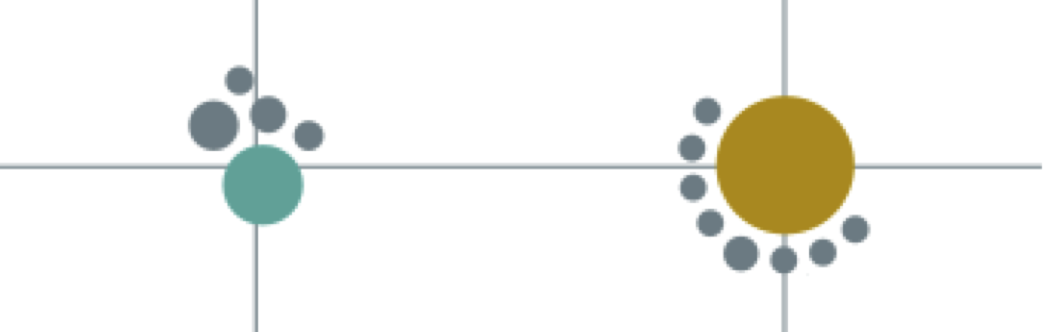
\includegraphics[width=.5\textwidth]{./grid-1}}

\newpage

\section{Travailler avec d'autres logiciels et exporter ses données}

\subsection{Vérifier les désignations VDJ avec d'autres logiciels}

Pour certaines études, il est  très important d'avoir les bonnes désignations VDJ.
Dans la liste des clones et dans le segmenteur, ces désignations sont écrites de manière
concise afin de gagner de la place.

\question{%
  Positionnez le curseur de la souris sur un des clones. La désignation
  complète de la séquence apparaît dans la barre de status, entre la
  grille et le segmenteur.}

Nous pouvons vérifier cette assignation par d'autres logiciels.

\question{Sélectionnez quelques clones.}
\question{%
\marginpar{Cela nécessite une connexion internet}
  Cliquez sur le triangle à droite du bouton \com{IMGT/V-QUEST} dans la
  partie en bas à gauche. Les séquences des clones sélectionnés sont
  envoyées à IMGT/V-QUEST.}
\question{Ensuite, cochez la case \com{5'V/D/3'J}. Dans le segmenteur, les jonctions
  V(D)J qui ont été définies par IMGT/V-QUEST sont soulignées.}
\question{%
  Vous pouvez aussi envoyer directement les séquences sur IMGT/V-QUEST
  ou IgBlast en cliquant sur le bouton portant leur nom respectif.}
  vous pouvez remarquer que les données renvoyées par IMGT/V-QUEST sont disponible en cliquant sur sur le textit{i} bouton ce qui vous permet de comparer les annotations du logiciel originel et celle d'IMGT/ V-QUEST.       

\bigskip

Il arrive parfois que Vidjil fasse des erreurs dans la désignation VDJ.
Dans ce cas, vous êtes fortement invités à nous en faire part et nous
essaierons d'améliorer l'algorithme de désignation.

\question{Utilisez le bouton \com{get support}  situé dans le menu \com{help}.
  Un mail pré-composé s'ouvre avec les références des données
  que vous visualisez tout comme des clones sélectionnés.}

Même sans utilser le bouton \com{get support}, une bonne habitude est
d'envoyer l'adresse complète se trouvant dans votre navigateur web,
telle que \url{http://app.vidjil.org/?set=3241&config=39&plot=v,size,bar},
quand vous voulez discuter avec des collègues ou avec nous de vos données
ou de vos analyses.

\bigskip

Supposons que vous souhaitiez
changer la désignation V(D)J.


\question{%
  Dans la liste des clones, cliquez sur le «~\textit{i}~» à droite du clone dont
  vous voulez changer le nom. Dans la partie Segmentation, cliquez sur
  le bouton \com{edit}. Faites-les modifications souhaitées.}

Attention : aucune des modifications effectuées (changement de nom,
regroupement de clones, apposition de tags) ne sont sauvegardées
automatiquement.
Il faut le faire manuellement soit en cliquant sur \com{save patient} dans le
menu tout en haut à gauche (là où le nom du «~patient~» est écrit), soit avec
le raccourci clavier \texttt{Ctrl+S}.
Cependant, pour ce jeu de démonstration, il n'est pas possible de faire de
sauvegarde. Vous pourrez en revanche sauvegarder les échantillons qui vous
appartiennent !

\subsection{Export de données}

\question{%
  Pour générer des rapports imprimables,
  dans le menu \com{import/export}, cliquez sur les deux entrées commençant par
  \com{export report}. Quelles sont les différences entre les deux~?}
\question{
  Sélectionnez quelques clones. Ensuite, dans le menu \com{import/export},
  choissisez \com{export fasta}. Que se passe-t-il~?}


\question{Ouvrez le menu \com{import/export} et cliquez sur \com{export svg}.
  Le fichier ainsi généré décrit tous les clones (désignation V(D)J, abondance à chaque échantillon)
  et peut être ouvert par n'importe quel tableur pour de plus amples analyses.}  

\question{Ouvrez de nouveau le menu \com{import/export} et cliquez sur \com{export svg}.
  Ceci exporte la vue du graphe ou de la grille.
  La fichier ainsi généré peut être ouvert et édité par tout logiciel d'image vectoriel comme Inkscape.
  
}  

\vfill
\flushright \it Aurélien Béliard, Aurélie Caillault, Mathieu Giraud, Tatiana Rocher, Mikaël Salson, Florian Thonier, 
\\ \texttt{contact@vidjil.org}

\end{document}
